 %% Copernicus Publications Manuscript Preparation Template for LaTeX Submissions
%% ---------------------------------
%% This template should be used for copernicus.cls
%% The class file and some style files are bundled in the Copernicus Latex Package, which can be downloaded from the different journal webpages.
%% For further assistance please contact Copernicus Publications at: production@copernicus.org
%% http://publications.copernicus.org/for_authors/manuscript_preparation.html

%% Please use the following documentclass and journal abbreviations for discussion papers and final revised papers.

%% 2-column papers and discussion papers
\documentclass[amtd, manuscript]{copernicus}

%% \usepackage commands included in the copernicus.cls:
%\usepackage[german, english]{babel}
%\usepackage{tabularx}
%\usepackage{cancel}
%\usepackage{multirow}
%\usepackage{supertabular}
%\usepackage{algorithmic}
%\usepackage{algorithm}
%\usepackage{amsthm}
%\usepackage{float}
%\usepackage{subfig}
%\usepackage{rotating}
\usepackage{fancyvrb}
\usepackage{comment}
%\usepackage{draftwatermark}
%\SetWatermarkLightness{0.95}
%\SetWatermarkScale{1}

\usepackage[normalem]{ulem} %% Added by Hamid

% uncomment to include stuff in standard comment-environment
%\includecomment{comment}

\begin{document}

%\title{The impact of various parameters on statistical properties of
%  dispersed atmospheric trace gases as inferred from camera images: a
%  modelling sensitivity study}
\title{Not THE title: Plume velocity determination: comparison of methods}

% \Author[affil]{given_name}{surname}

\Author[1]{Arve}{Kylling}
\Author[2]{Jonas}{Gliss}
\Author[1]{Hamidreza}{Ardeshiri}
\Author[1]{Massimo}{Cassiani}
\Author[3]{Anna Solvejg}{Dinger}
\Author[4]{Soon-Young}{Park}
\Author[1]{Ignacio}{Pisso}
\Author[1]{Norbert}{Schmidbauer}
\Author[1]{Kerstin}{Stebel}
\Author[1]{Andreas}{Stohl}

\affil[1]{NILU - Norwegian Institute for Air Research, NO-2007 Kjeller, Norway}
\affil[2]{Norwegian Meteorological Institute, Oslo, Norway}
\affil[3]{PGS, Oslo, Norway}
\affil[4]{Center for Earth and Environmental Modeling Studies, Gwangju
  Institute of Science and Technology, Gwangju, Republic of Korea}

%\runningtitle{Statistical properties of dispersed atmospheric trace gases}
\runningtitle{Velocity from UV camera observations of SO$_2$}

\runningauthor{Kylling et al.}

\correspondence{Arve Kylling (arve.kylling@nilu.no)}

\received{}
\pubdiscuss{} %% only important for two-stage journals
\revised{}
\accepted{}
\published{}

%% These dates will be inserted by Copernicus Publications during the typesetting process.
\def\veloana{0}
\def\tomography{0}

\firstpage{1}

\maketitle

\begin{abstract}
To come
\end{abstract}

%\copyrightstatement{TEXT}

%\clearpage
%\newpage

\newpage

\textcolor{red}{
  NOTES\\
  \\
  \\
  \begin{itemize}
  \item
    Vary distacne between PCS-lines.
  \item
    Plot lag shift
  \item
    Compare pure optical flow and optical flow with histogram
  \item
    Is  optical flow underestimating?
\item Have a little older plume so that the
  range of detectable AA values covers a little more pixels in the
  vertical (maybe Hamid et al need to increase the emissions in that
  case, so that we get enough AA in the older plume).
\item
\item background wind velocity (e.g. between 1 and 10 m/s)
\item background wind direction (e.g. simulate plume / camera CFOV
  angle range of e.g. 70 to 110 degrees)
\item turbulent intensity (i.e. spectrum of velocity vector
  magnitudes and orientations -> could be interesting to see how the
  smoothness constraint of optical flow algorithms impacts the pixel
  based velocity estimates).
\item It could be also interesting to see a convective version of
  the plume at very low velocities and investigate if the optical
  flow can capture the decrease in velocity between the centre and
  the edges of the plume.
\item Also, if we have a higher signal in the aged plume (i.e. AA of the
  order of 0.1-1.0), then the very young plume probably suffers
  saturation and hence shows little contrast for the velocity
  retrieval. Could be interesting to see how this impacts the optical
  flow velocities too.
\end{itemize}
}

\introduction
\textcolor{red}{Describe earlier work}


\textcolor{red}{Describe what is done in this paper}


The paper ends with the conclusions in section~\ref{sec:conclusions}.


\section{Methods}
\label{sec:Methods}

The large eddy  and the radiative transfer simulations have been
described in detail by \citet{Kylling2020} and are briefly summarized
here for completeness.

\subsection{Large eddy simulation (LES) }
\label{sec:LES}
In LES the large scales of the turbulent flow are
explicitly simulated while a low-pass filter is applied to the
governing equations to remove the small scales information from the
numerical solution. The effects of the small scales  are then
parameterized by means of a sub-grid scale (SGS) model
\citep[e.g.][]{Deardorff-1973, Moeng-1984,
  Pope-2000,Celik_etal-2009}.
We calculated the 3D SO$_2$ concentrations as a function of time in a
three dimensional domain of $1000~$m~$\times~375$~m~$\times~250$~m in
the along wind ($x$), crosswind ($y$) and vertical ($z$) directions
respectively, was simulated with a grid resolution of $nx \times ny
\times nz = 1024 \times 384 \times 256$. Here $nx, ny, nz$ are the
number of grid nodes in along wind, crosswind and vertical directions,
respectively. This implies that the size of a grid cell is $0.98^3 \,
$m$^3 \approx 1\, $m$^3$. The release points were located at $25\,$m
and $150\,$m
above the ground.  A total of 100 time frames were calculated with a
time resolution of 1.5625~s.
We used the Parallelized Large-Eddy Simulation Model \citep[PALM,
][]{Raasch2001,Maronga2015} to solve the filtered, incompressible
Navier-Stokes equations in Boussinesq-approximated form, at infinite
Reynolds number.
For further information on the model set-up see
\citet{Ardeshiri2019}.

\textcolor{red}{WHAT IS THE WIND SPEED?}

\subsection{Radiative transfer simulations}
The 3D MYSTIC Monte Carlo radiative transfer model was used to
calculate UV camera images \citep{Mayer2010,Emde2010,Buras2011a,Kylling2020}.
To simulate a camera with a prescribed number of pixels, MYSTIC was run
in backward mode and calculated the  radiation impinging the camera
plane defined by the location of the camera within a 3D domain and the
camera viewing direction. Camera images were calculated for
wavelengths suitable for the detection of SO$_2$.
For each camera pixel, spectra were calculated for wavelengths between
300 and 350.5~nm with a spectral resolution of 0.1~nm in order to
capture the fine structure of the SO$_2$ cross section. The spectra were
weighted with spectral response functions (about 10~nm width)
representing cameras with mounted on-band
(sensitive to SO$_2$ absorption, centred at 310~nm) and off-band (barely sensitive to SO$_2$
absorption, centred about 330~nm) filters similar to those described
by \citet{Gliss2018}. Quantum efficiency of the detector and
geometrical effects related to lens/camera optics are not included in
the camera simulations.
SO$_2$ plume concentrations were taken from the LES simulations and
the spectrally dependent SO$_2$ absorption cross section was from
\citet{Hermans2009}.
For representing the ambient atmosphere the mid-latitude summer atmosphere of
\citet{Anderson1986} was used. The surface albedo is small in the UV
for non-snow covered surfaces and was thus set to zero. Aerosols were
not included. The solar zenith angle was 40$^{\circ}$ and the
sun azimuth angle was perpendicular to the camera viewing direction,
see Fig.~\ref{fig:ExpSetup}.

As in \citet{Kylling2020} cameras at four different locations were
simulated. Their location and viewing geometries are summarized in
Table~\ref{tab:CameraInfo} and a bird's eye view is shown in Fig.~\ref{fig:ExpSetup}.
\begin{table}[t]
  \caption[]
          {\label{tab:CameraInfo}
            Location and geometric specification of the four simulated cameras.
            All cameras  were placed 1 meter above the
            surface. Adopted from  \citet{Kylling2020}.}
          \begin{tabular}{ccccc}
            \tophline
            Camera & FOV & Viewing elevation &          No. of pixels. & x-location \\
            & (degrees)  &  (degrees) & (horizontal$\times$vertical)& (m)\\
            \middlehline
            A & 46$^\circ\times$10$^\circ$ & 5.73$^\circ$ & 400$\times$88 &  500   \\
            B & 11.5$^\circ\times$30$^\circ$ & 30.7$^\circ$ & 100$\times$264 &  500   \\
            C & 11.5$^\circ\times$30$^\circ$ & 30.7$^\circ$ & 100$\times$264 &  700   \\
            D & 11.5$^\circ\times$30$^\circ$ & 30.7$^\circ$ & 100$\times$264 &  900   \\
            \bottomhline
          \end{tabular}
\end{table}
% python PlotLESNetCDF.py FIG = 'fig_02'
\begin{figure}[!htb]
  \begin{center}
    \includegraphics[width=0.495\textwidth]{../text//figs/BirdEyeXYLES005_V2.png}
    \caption{\label{fig:ExpSetup} Bird's eyes view of the
      3D domain (black square) and the SO$_2$ plume location
      within the camera A domain simualtion (red square).
      The UV camera is located where the two green or blue lines
      intersect. The lines indicate  the cameras' horizontal field-of-view.
      The direction of the incoming sun ray is indicated by the yellow line.
      The plume column density is included for illustrative purposes.
      Adopted from  \citet{Kylling2020}.
    }
  \end{center}
\end{figure}
Camera A views the plume from its release point and
about 200~m downwind. For camera A the plume release altitude was 25~m
and the camera A thus have low angle viewing elevations, see
Table~\ref{tab:CameraInfo}.
For cameras B, C and D the plume release altitude was 150~m and these
cameras thus  have a larger viewing elevation. Camera A is placed at the same x-direction
location as camera~A, but as a smaller horizontal FOV to focus on the
more mature parts of the plume. Cameras C and D are placed further
downwind and views more dispersed parts of the plume about 300 and
500~m downwind from the release point, respectively.

From the on and off-band radiances,  $I_{\textit{on, off},M}$, the
apparent absorbance was calculated \citep{MoriT2006a,Lubcke2013}
\begin{eqnarray}
\label{Eq:AA}
\tau = \tau_{\textit{on}}  - \tau_{\textit{off}} = -\ln \frac{I_{\textit{on},M}}{I_{\textit{on},0}}+\ln\frac{I_{\textit{off},M}}{I_{\textit{off},0}}
     = \ln \left(\frac{I_{\textit{off},M}}{I_{\textit{on},M}} \frac{I_{\textit{on},0}}{I_{\textit{off},0}}\right),
\end{eqnarray}
where $I_{\textit{on,off},0}$ are the background radiances without the SO$_2$ plume.
The background images were calculated similar to the plume images, but with the
SO$_2$ concentration set to zero.

The LES voxel resolution is about 1~m$^3$ which at a distance of 250~m
(roughly distance between cameras and plume) corresponds to
0.004~rad=0.23$^\circ$. The number of pixels in the simulated images
were set to oversample the spatial resolution of the LES simulations by about a
factor of two. The number of simulated pixels are  smaller than found
in real cameras; for example  \citet{Dinger2018} used cameras with
1392$\times$1040 pixels and a field of view (FOV) of
14.7$^\circ\times$11.1$^\circ$. The memory and computer time
requirements increase with the numberof pixels, making simulations for
so many pixels not currently feasible. Furthermore, the LES input
would need to be at higher spatial resolution to justify simulation of
cameras with more pixels.

The radiative transfer simulations were run on a Linux cluster
utilizing 10 processors in parallel with each process needing about
10~GB of memory. For each pixel and wavelength 2000 photons
were traced to ensure that the statistical noise of the MYSTIC Monte
Carlo simulations were  about the same order of magnitude as the
measurements ($\approx$~1\%).

\subsection{Velocity analysis}

\textcolor{red}{Describe PCS lines}

\subsubsection{Velocity from optical flow}
\textcolor{red}{Describe how it is calculated. Mention that plume flow
  direction is also derived.}


\subsubsection{Velocity from cross correlation}
\textcolor{red}{Describe how it is calculated}


\section{Results}
\subsection{Velocity analysis: synthetic data}
In Fig.~\ref{fig:Fig_Image_LocA} is shown apparent absorbances for the
eight time steps used for the velocity analysis of camera A images.
% source velocity.sh
% convert -append output_new/LocA_250/aa_img* ../Velocity_paper/Fig_Image_LocA.png
\begin{figure}[!htb]
  \begin{center}
    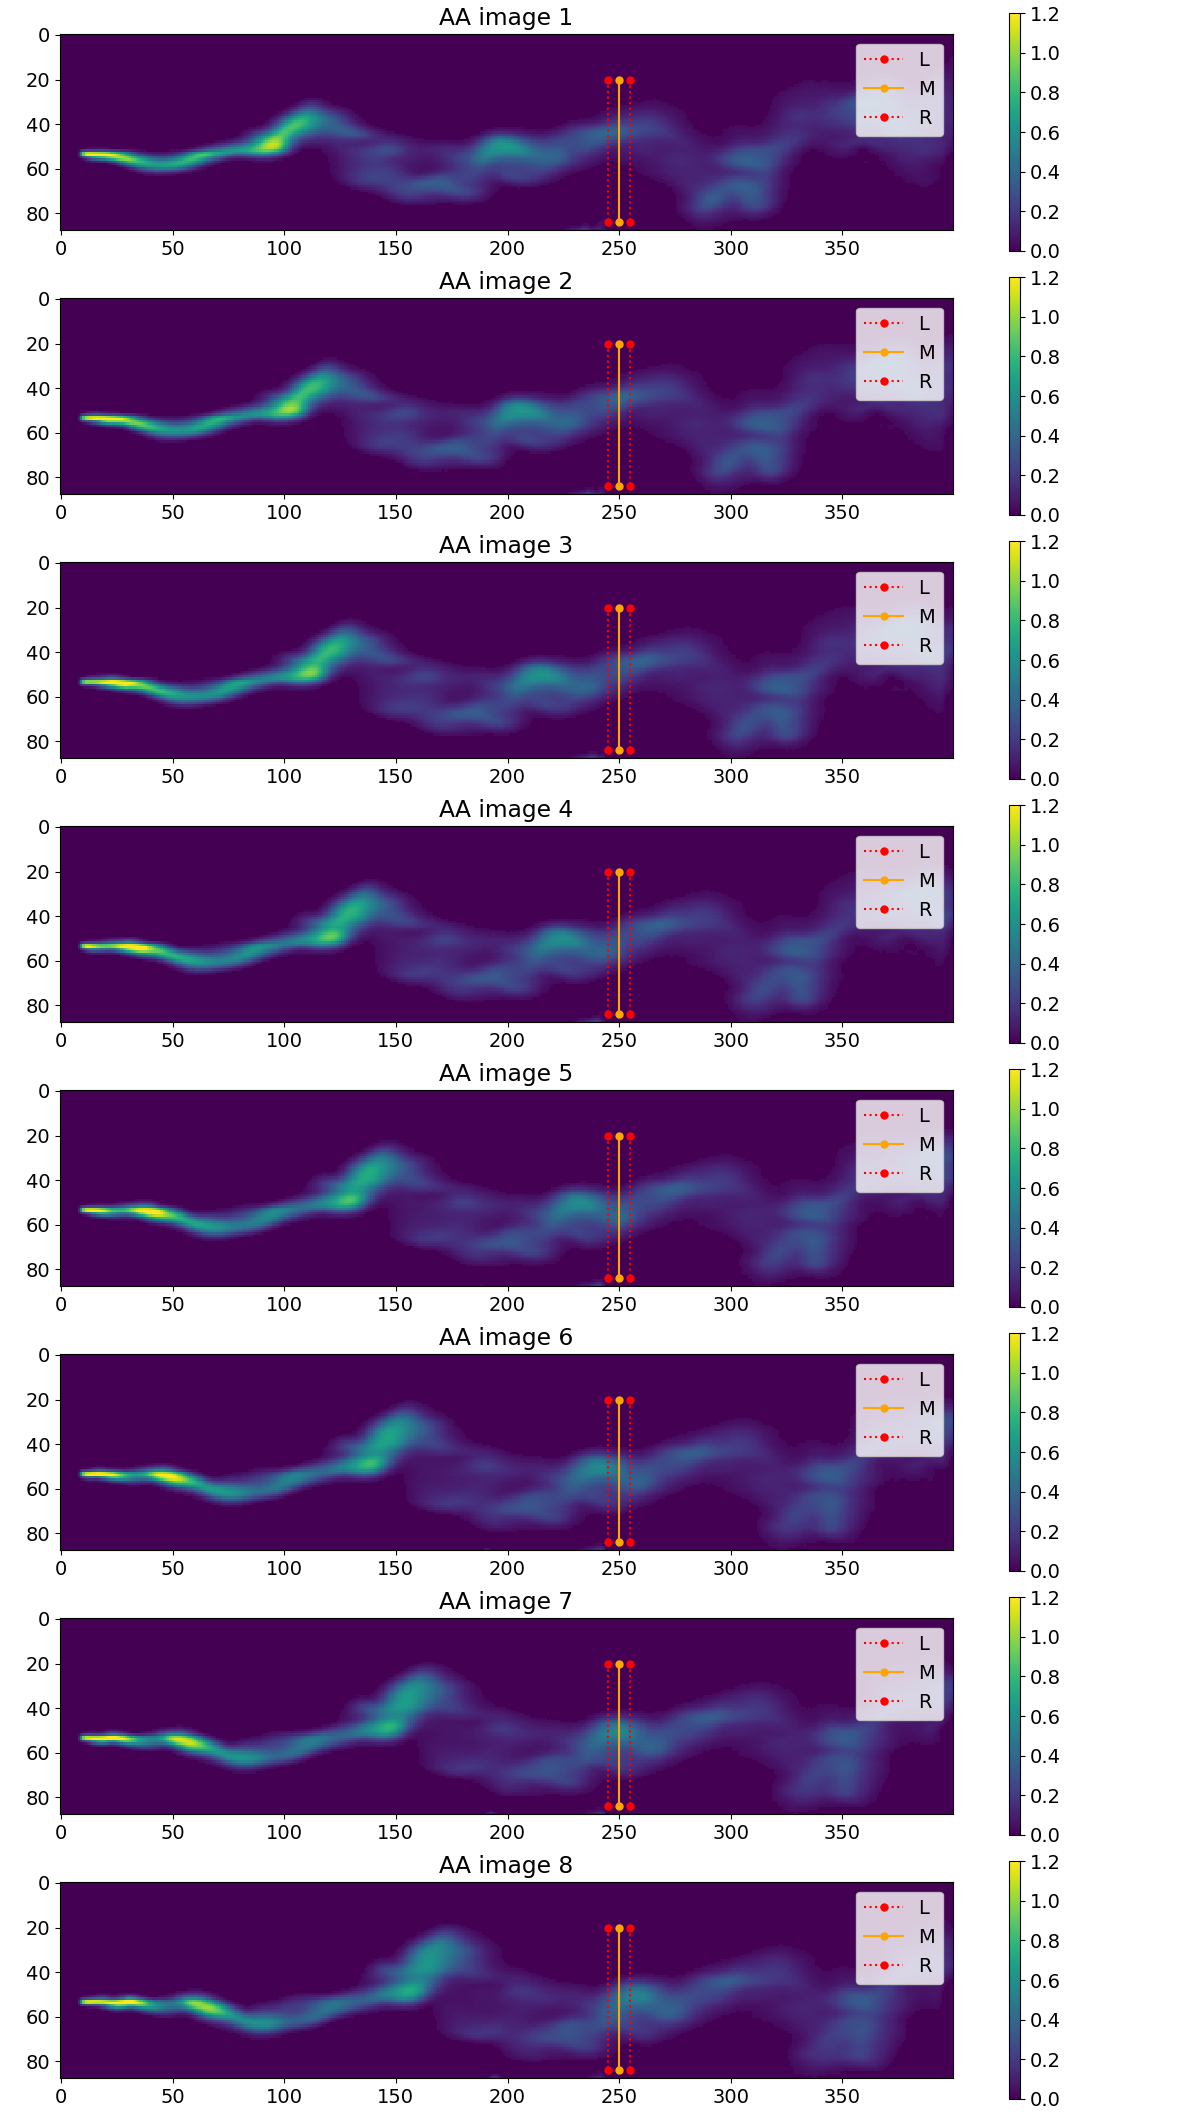
\includegraphics[width=0.55\textwidth]{Fig_Image_LocA.png}\\
    \caption{\label{fig:Fig_Image_LocA}
      The apparent absorbance as derived from  camera A images.
      The lines labelled M shows the PCS line used for the cross correlation
      velocity estimate. The lines labelled L and R are the left  and right
      boundaries of a rectangular box encompassing the  region used for the
      optical flow velocity analysis.
      Units on x- and y-axes are in pixels.
    }
  \end{center}
\end{figure}
The lines labelled M shows the PCS line used for the cross correlation
velocity estimate. The lines labelled L and R are the left  and right
boundaries of a rectangular box encompassing the  region used for the
optical flow velocity analysis. In Fig.~\ref{fig:Fig_Image_LocA} the
PCS line is at x pixel 250. Below, velocity results are presented with
the M-line at 100, 150, 200, 250, 300 and 350.

In Fig.~\ref{fig:Fig_Image_LocV} is shown the apparent absorption
images from cameras at locations B (top row), C  (middle row) and D
(bottom row).
% convert +append output_new/LocV01_50/aa_img* ../Velocity_paper/Fig_Image_LocV01.png
% convert +append output_new/LocV02_50/aa_img* ../Velocity_paper/Fig_Image_LocV02.png
% convert +append output_new/LocV03_50/aa_img* ../Velocity_paper/Fig_Image_LocV03.png
\begin{figure}[!htb]
  \begin{center}
    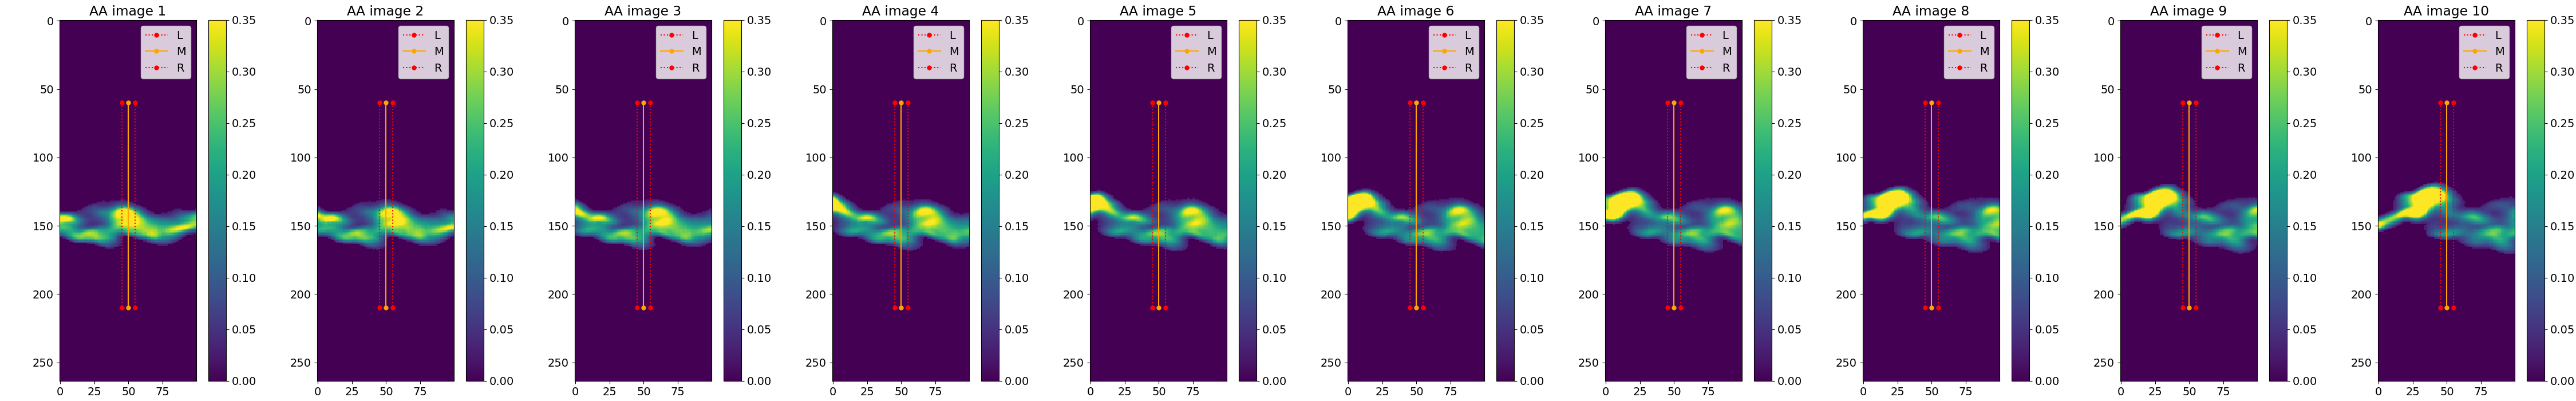
\includegraphics[width=0.99\textwidth]{Fig_Image_LocV01.png}\\
    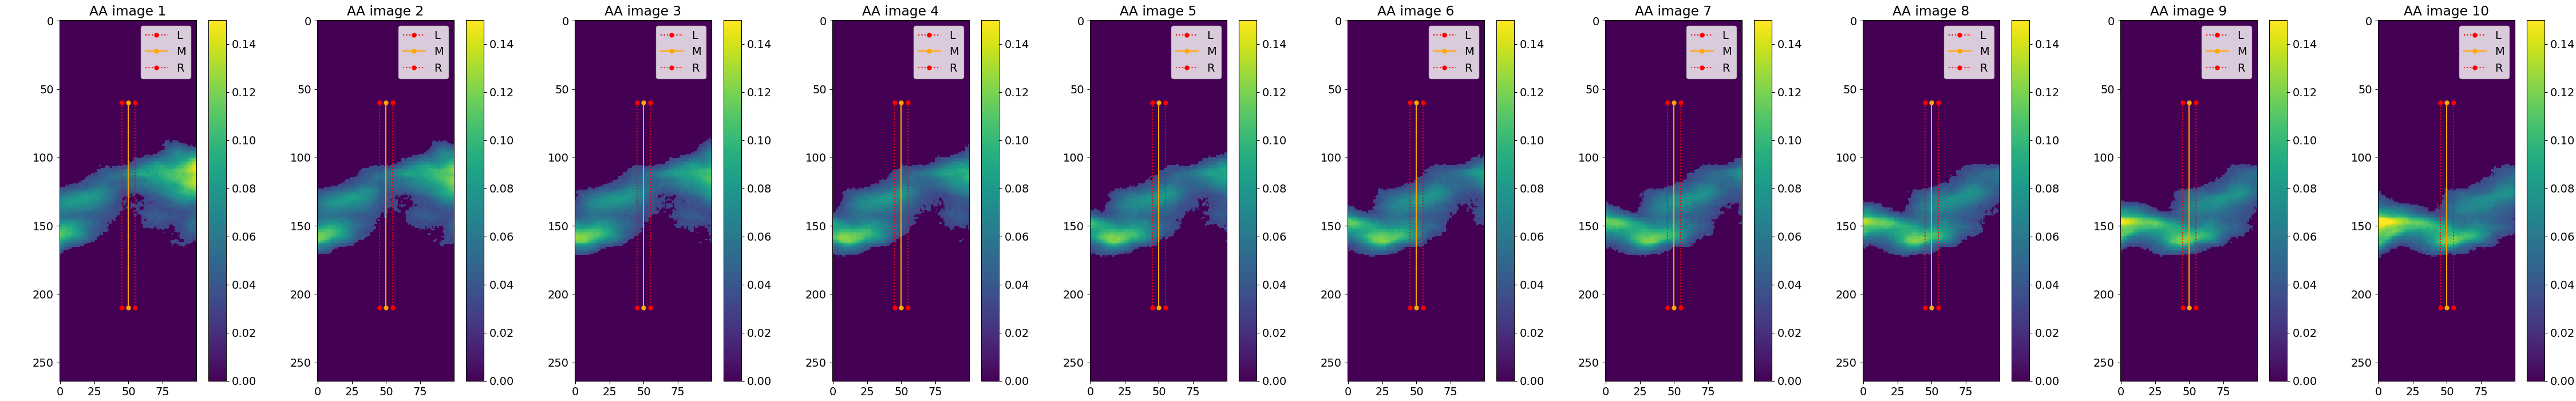
\includegraphics[width=0.99\textwidth]{Fig_Image_LocV02.png}\\
    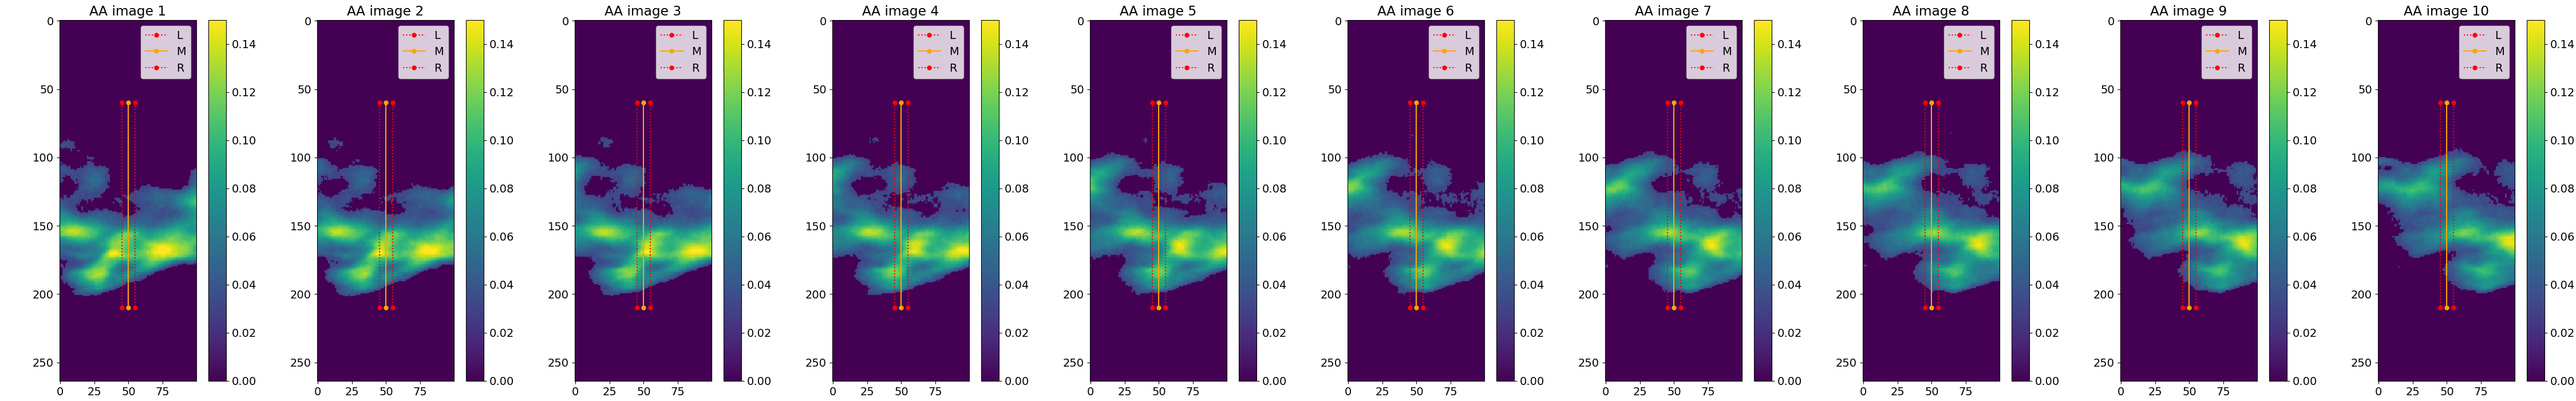
\includegraphics[width=0.99\textwidth]{Fig_Image_LocV03.png}\\
    \caption{\label{fig:Fig_Image_LocV}
      Apparent absorption (AA) images from cameras at locations B (top row), C
      (middle row) and D (bottom row) and time steps 1 to 10 (columns
      1 to 10). PCS lines similar as in Fig.~\ref{fig:Fig_Image_LocA}.
      Note different scales on colorbars.
    }
  \end{center}
\end{figure}
A total of ten time steps were used for these cameras and the M-line
was located at 10, 20, 30, 40, 50, 60 and 70.

The velocities  at different PCS lines using the cross correlation and
optical flow methods are shown for camera A in
Fig.~\ref{fig:Fig_Velo_LocA} and cameras B, C and D in
Fig.~\ref{fig:Fig_Velo_LocV}.
% source velocity.sh
%
\begin{figure}[!htb]
  \begin{center}
    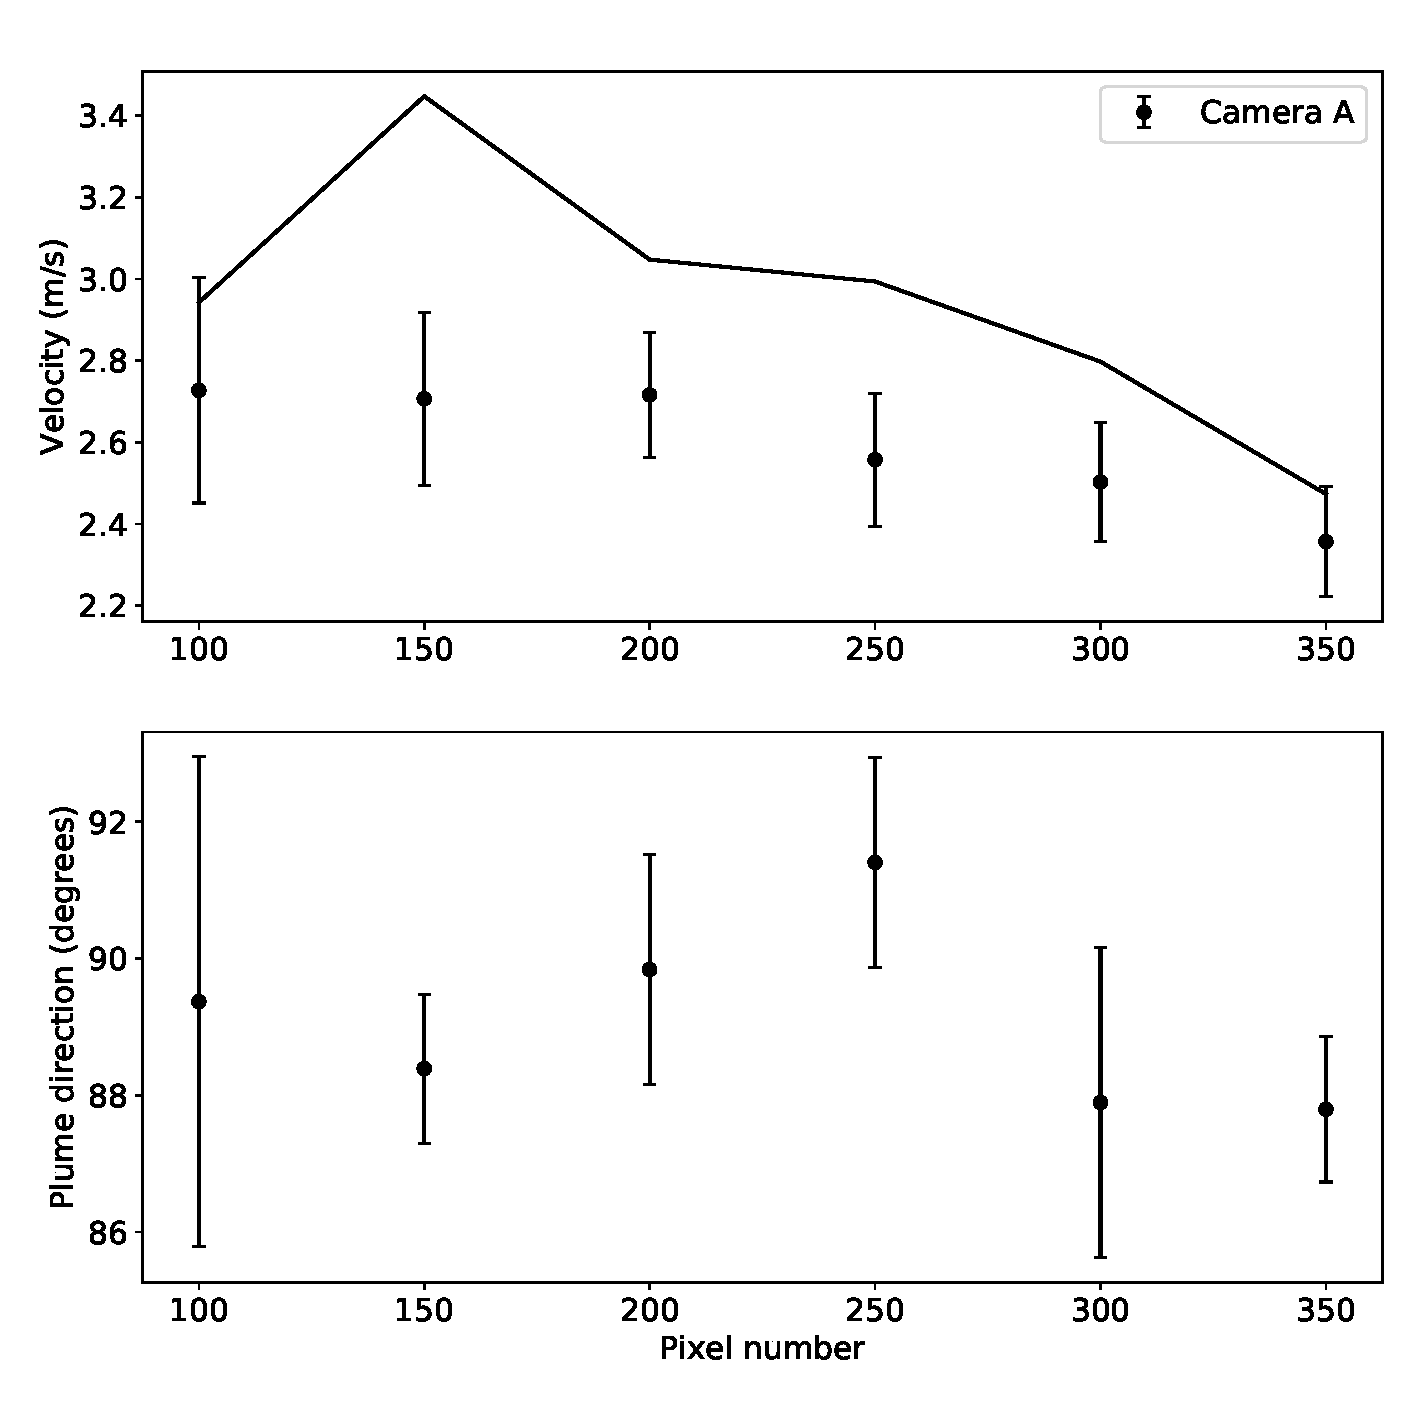
\includegraphics[width=0.75\textwidth]{Fig_Velo_LocA.pdf}\\
    \caption{\label{fig:Fig_Velo_LocA}
      (Top) The average plume velocity as determined by the optical
      flow method (dots) where error bars indicate the standard
      deviation. The velocity is determined at a plume cross section
      at the pixel given at the x-axis. The solid line is the plume
      velocity determined using cross correlation analysis.
      (Bottom) The average plume direction and standard deviation
      indicated by error bars. Determined with the optical flow analysis.
    }
  \end{center}
\end{figure}
\begin{figure}[!htb]
  \begin{center}
    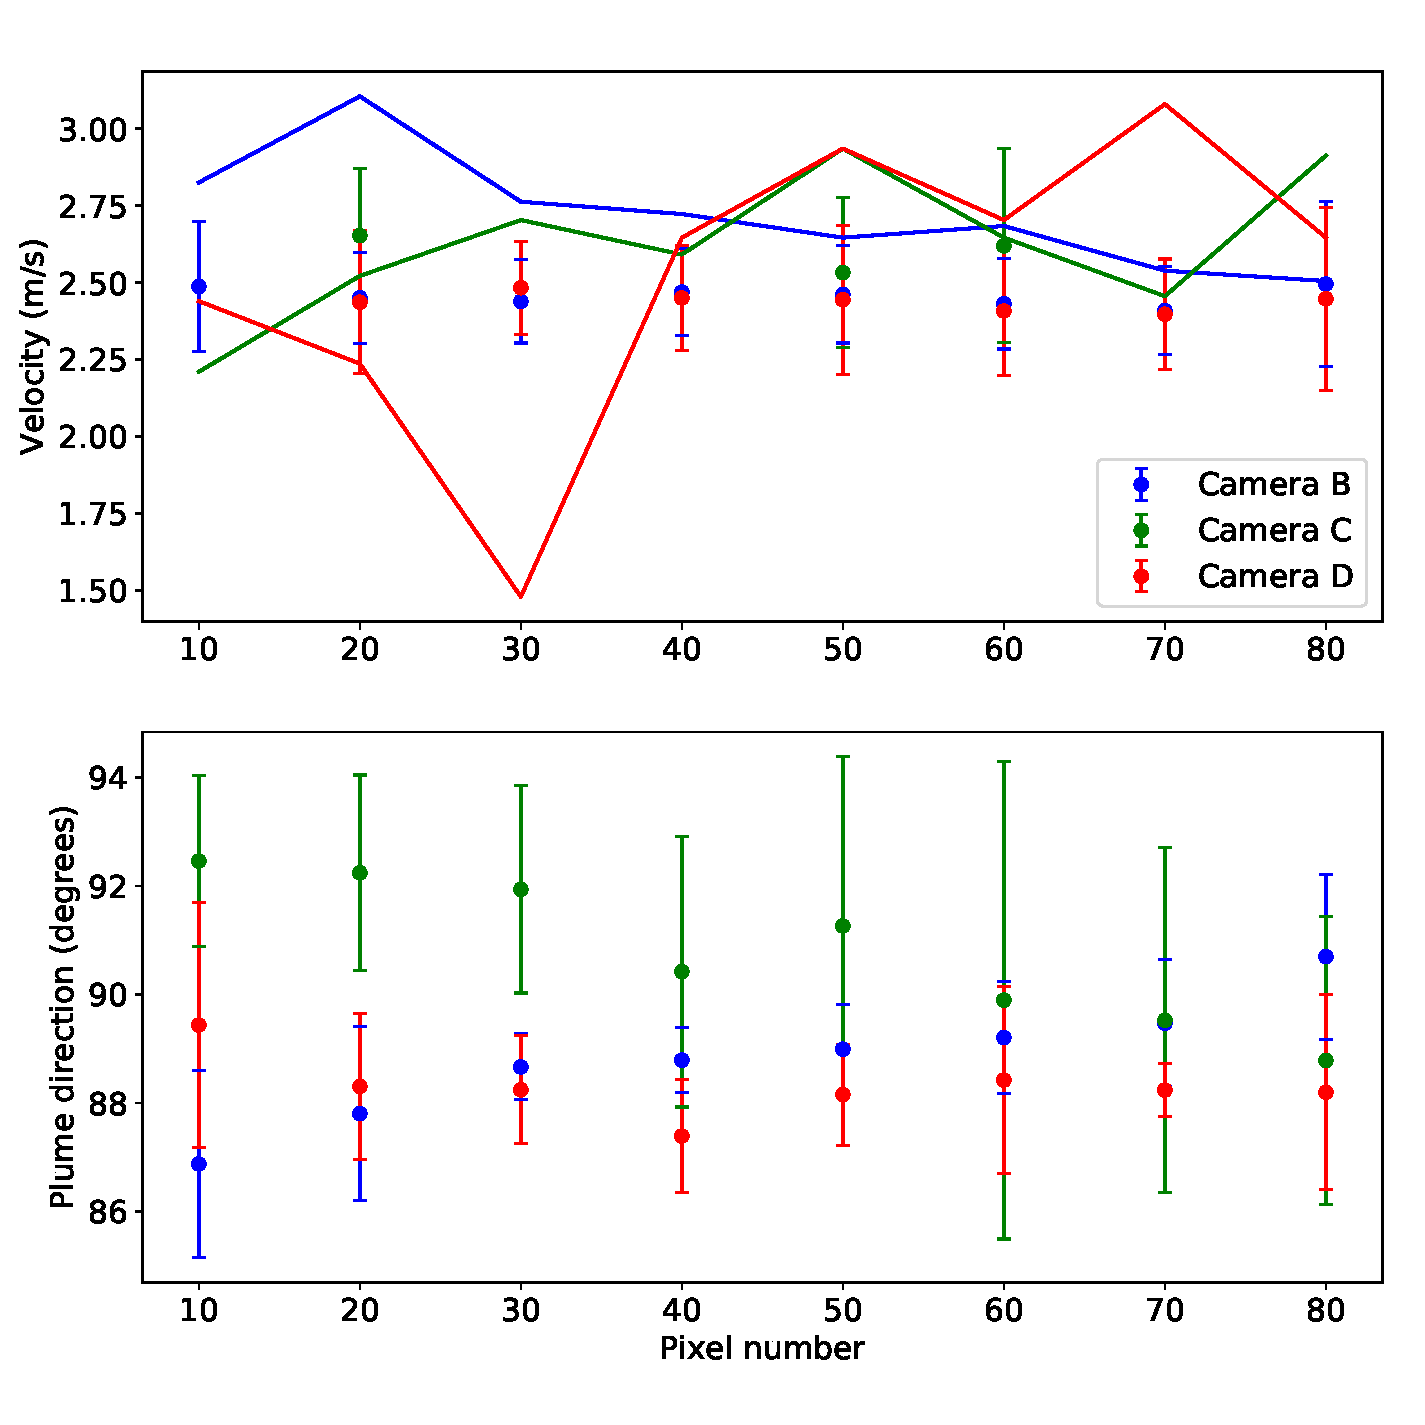
\includegraphics[width=0.75\textwidth]{Fig_Velo_LocV.pdf}\\
    \caption{\label{fig:Fig_Velo_LocV}
      Similar to Fig.~\ref{fig:Fig_Velo_LocA}, but for cameras B,
      C and D.
    }
  \end{center}
\end{figure}
Also shown in Figs.~\ref{fig:Fig_Velo_LocA} and
\ref{fig:Fig_Velo_LocV} are the plume directions as derived from the
optical flow.

\textcolor{red}{
  Some velocities missing because:
  }
\begin{Verbatim}
plumespeed.py(l3088,local_flow_params()): Aborting histogram analysis:
Multi-Gauss fit yielded additional Gaussian exceeding significance
thresh of 0.2 in histo of orientation angles

Significance: 30.67963866968083 %
Significance: 31.873164606888327 %
Significance: 23.06423881656792 %
Significance: 35.02810714760371 %
Significance: 61.6043930700684 %
Significance: 28.69744270222855 %
Significance: 59.029779606658074 %
Significance: 30.697942504522068 %
Significance: 21.73517476305695 %

Limit hard-coded to 0.2 in plumespeed.py

\end{Verbatim}



\subsection{Velocity analysis: measured data}
\textcolor{red}{Use continuous release data from Rena and/or data from
Stromboli}

\conclusions  %% \conclusions[modified heading if necessary]
\label{sec:conclusions}

%% use this section when having only software code available
\codeavailability{The libRadtran software used for the radiative
  transfer simulations is available from \url{www.libradtran.org}. The
  PALM model system was used for the LES and it is available from
  \url{palm.muk.uni-hannover.de/trac}. The ImageJ software is
  available from \url{https://imagej.nih.gov/ij/} and the FracLac
  plugin from
  \url{https://imagej.nih.gov/ij/plugins/fraclac/FLHelp/Introduction.htm}.}


\authorcontribution{AK performed the radiative transfer
  simulations. HA, MC and SYP were responsible for the LES. AK
  prepared the manuscript with contributions from all co-authors.}

\competinginterests{The authors declare that no competing interests are present.}

%% \disclaimer{TEXT} %% optional section

\begin{acknowledgements}
  The Comtessa project has received funding from the European Research
  Council (ERC) under the European Union's Horizon 2020 research and
  innovation programme under grant agreement no. 670462.
\end{acknowledgements}

%%
\bibliographystyle{copernicus}
\bibliography{archive,archive_tobe,archive_my_books,archive_misc,archive_special_issues}

\end{document}
